\documentclass[14pt]{beamer}
\usepackage[utf8]{inputenc}

\usepackage{utopia} %font utopia imported



\usetheme{Madrid}
\usecolortheme{default}

%------------------------------------------------------------
%This block of code defines the information to appear in the
%Title page
\title[Laser Training] %optional
{Laser Training}

\subtitle{Industra LABS Training Series}

\author[Simon Berka] % (optional)
{Simon Berka\inst{1} \and Industra LABS team\inst{2}}



\date[2019] % (optional)
{2019}



%End of title page configuration block
%------------------------------------------------------------



%------------------------------------------------------------
%The next block of commands puts the table of contents at the 
%beginning of each section and highlights the current section:

\AtBeginSection[]
{
	\begin{frame}
	\frametitle{Table of Contents}
	\tableofcontents[currentsection]
\end{frame}
}
%------------------------------------------------------------


\begin{document}

%The next statement creates the title page.
\frame{\titlepage}


%---------------------------------------------------------
%This block of code is for the table of contents after
%the title page
\begin{frame}
\frametitle{Table of Contents}
\tableofcontents
\end{frame}
%---------------------------------------------------------

\begin{frame}
\frametitle{Practical Test}
\centering
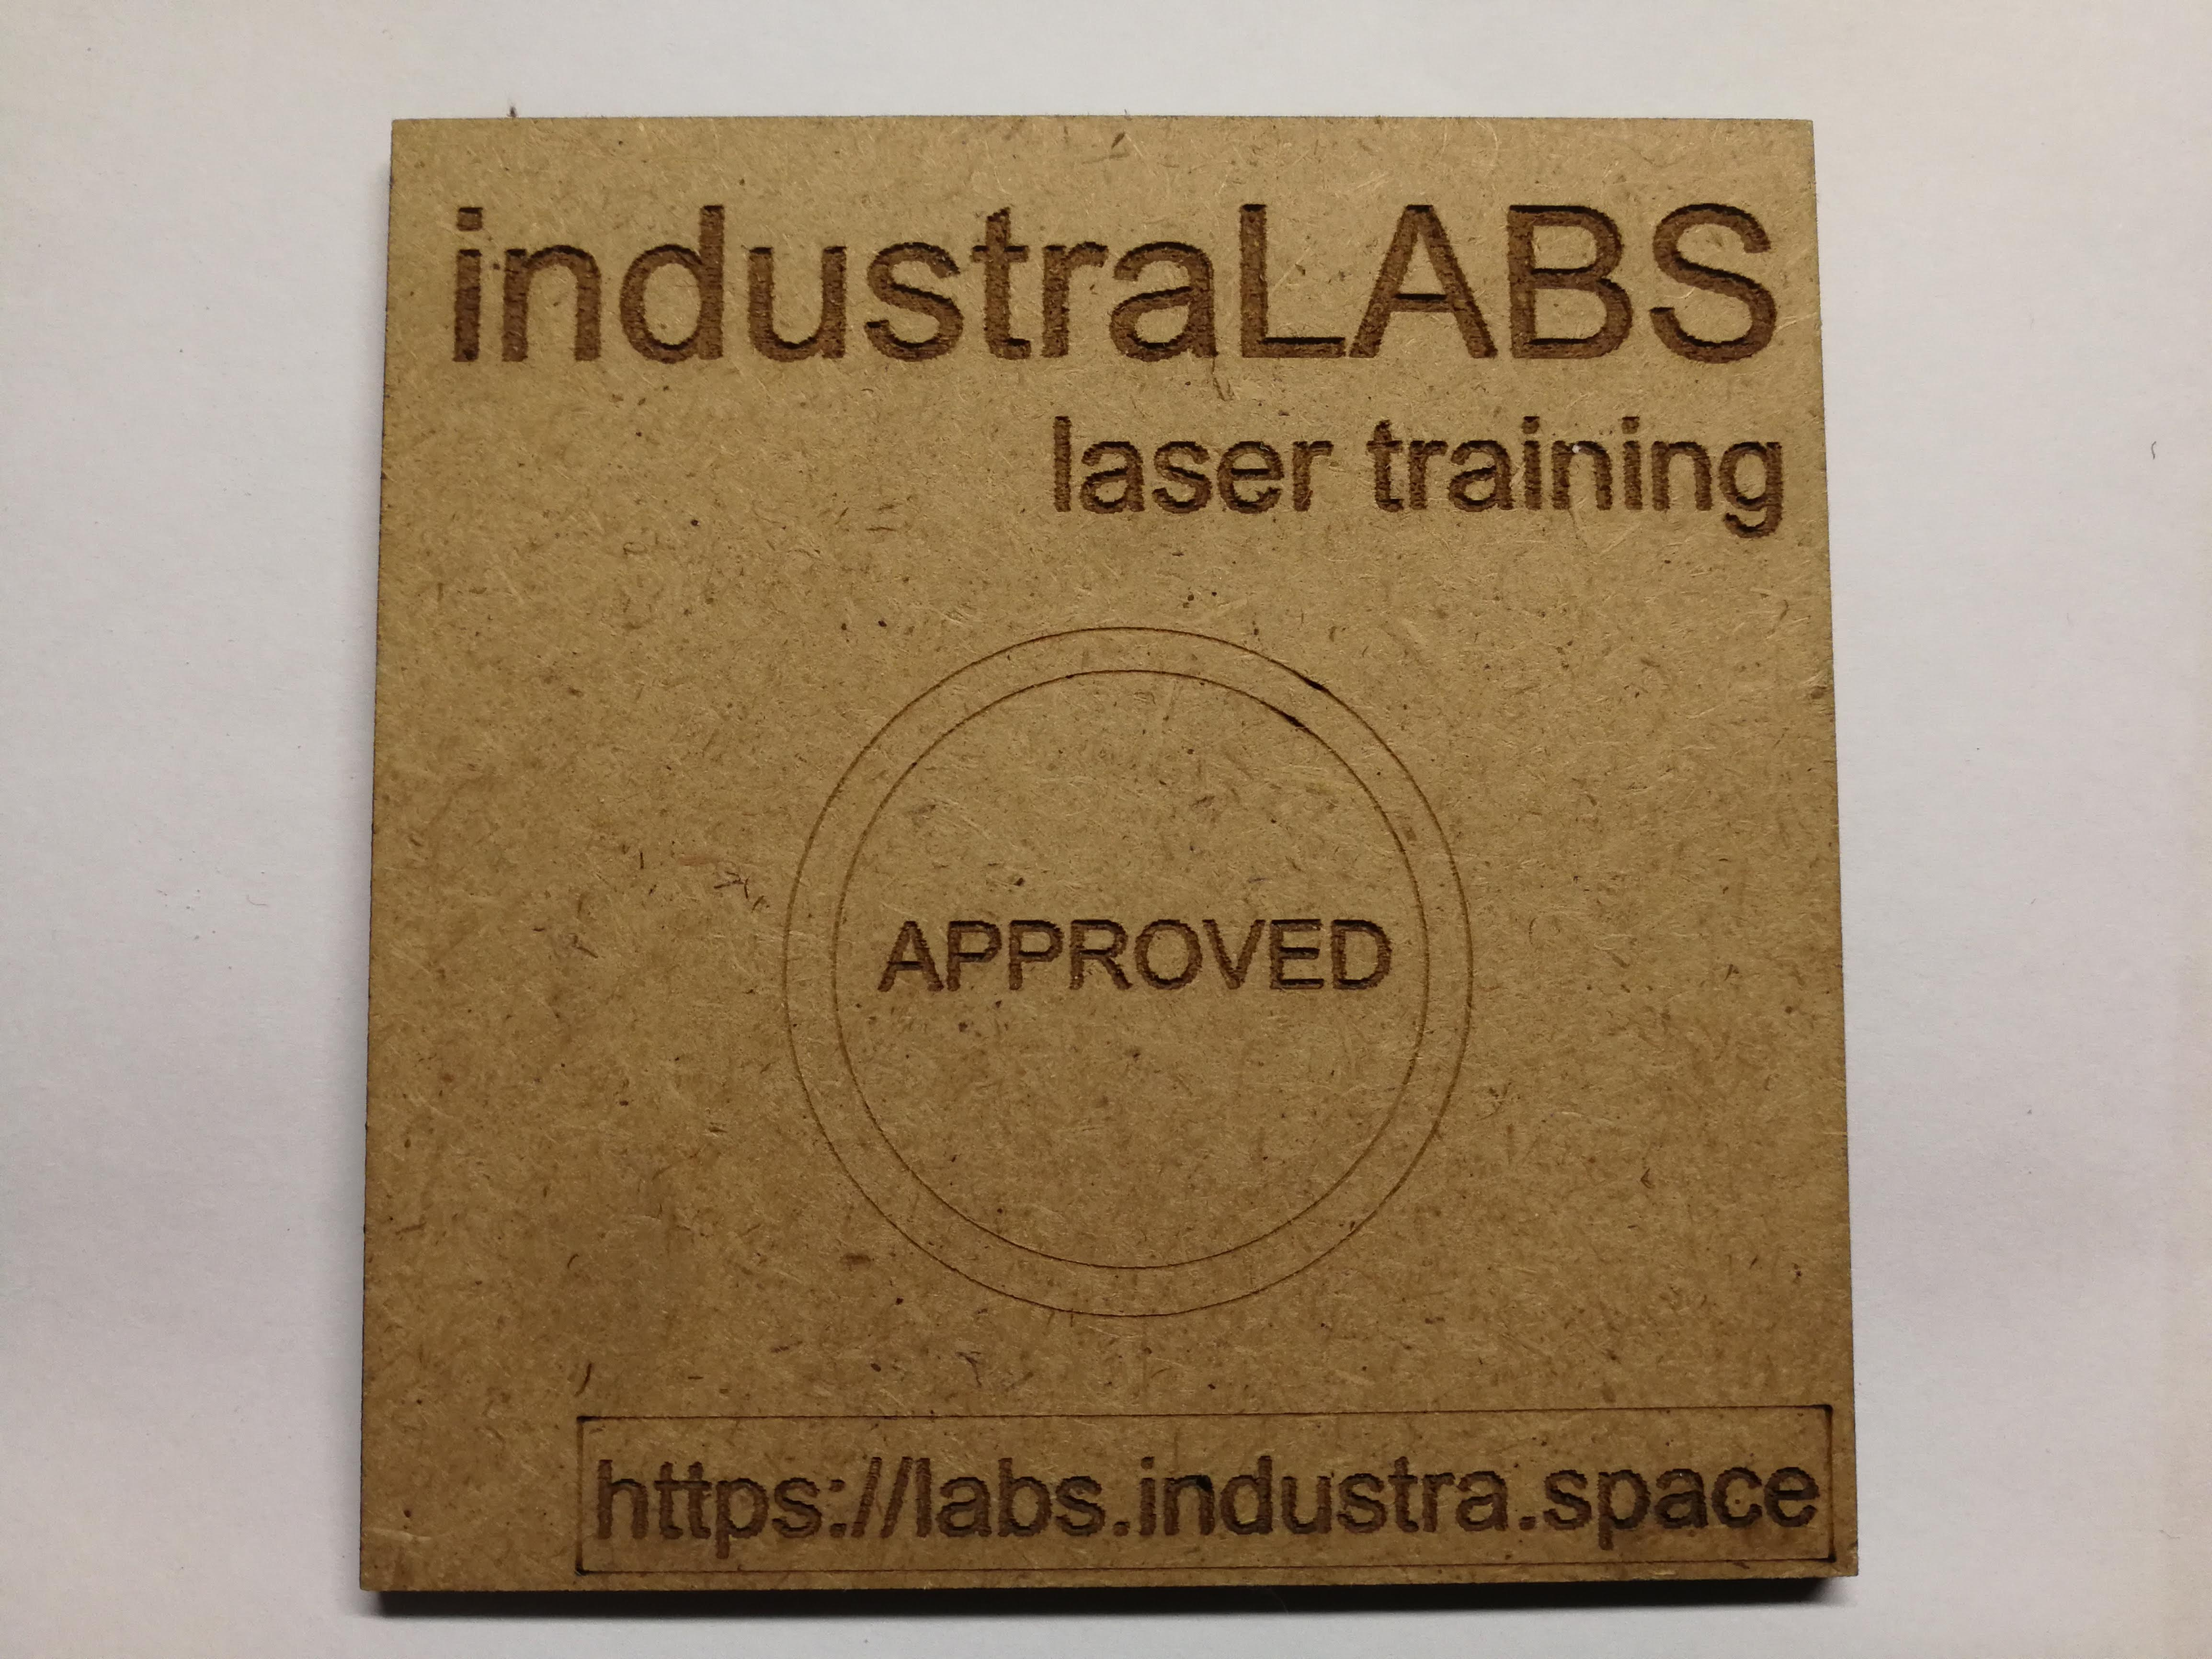
\includegraphics[scale=0.06]{imgs/approved.jpg}
\end{frame}

\section{Theory}

%---------------------------------------------------------
%Changing visivility of the text
\begin{frame}
\frametitle{The Laser}

\begin{block}{ThunderLaser Nova63}
\begin{itemize}
\item nonmetal cutting and engraving
\item 120W CO$_{2}$ laser
\item water cooling
%\item<2-> Text visible on slide 2
%\item<3> Text visible on slides 3
%\item<4-> Text visible on slide 4
\end{itemize}
\end{block}

\textbf{Basic laser workflow}
\begin{itemize}
	\item water cooling
	\item air assist
	\item fumes exhaust system
	
\end{itemize}
\end{frame}


%%% workflow chart



%%% workflow chart end



%---------------------------------------------------------
%%% Materials
\begin{frame}
\frametitle{Materials}


\begin{examples}
	\begin{itemize}
		\item wood
		\item HDF, MDF
		\item plywood (překližka)
		\item plexiglass
		\item cardboard, paper
		%\item<2-> Text visible on slide 2
		%\item<3> Text visible on slides 3
		%\item<4-> Text visible on slide 4
	\end{itemize}
\end{examples}




\end{frame}

%%% materials - not allowed
\begin{frame}
\frametitle{Materials}

\begin{alertblock}{Not Allowed}
	\begin{itemize}
		\item chlorine based materials (fumes)
		\item mirrors, copper (PCBs including) (laser reflection)
		\item hobbyglass (self healing)
		\item polystyrene foam
		\item ABS
	\end{itemize}
\end{alertblock}

\end{frame}



\begin{frame}
\frametitle{Laser Control Panel}

\centering
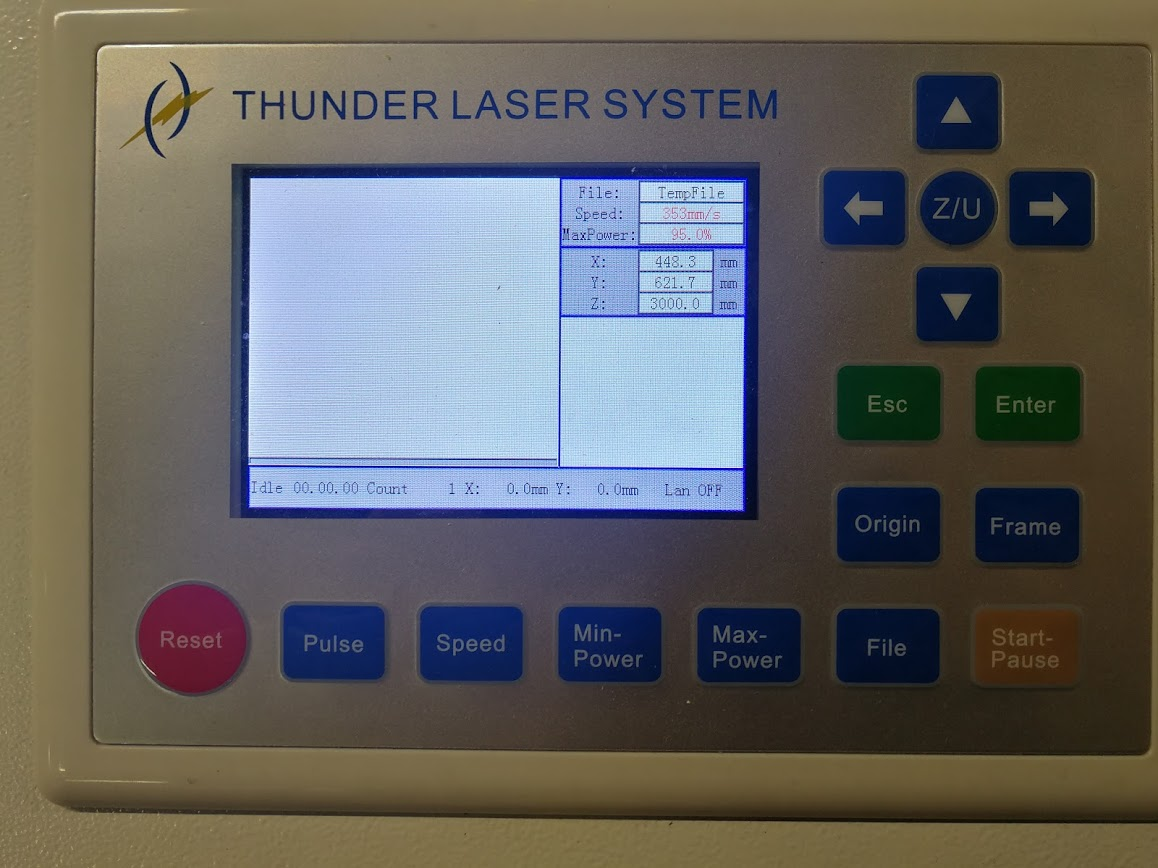
\includegraphics[scale=0.2]{imgs/laser_cp.jpg}

\end{frame}


%% SECURITY
\section{Security}
\begin{frame}
\frametitle{Security}

\begin{itemize}
	\item do not look into working laser all the time
	\item keep your hands out of the table area when moving table or laser head
	\item do not manipulate with any parts of laser (with exceptions like changing the laser head)
\end{itemize}

\begin{alertblock}{Use the RED STOP button in case of}
	\begin{itemize}
		\item fire
		\item unexpected behavior or sounds
	\end{itemize}
\end{alertblock}

\end{frame}


\begin{frame}
\frametitle{What is forbidden}

\begin{itemize}
	\item disable the air assist
	\item manipulate with laser frequency
	\item do not operate the laser without an explicit permission from the core team
	\item do not operate the laser from your own device (you can prepare LightBurn job on your machine, but you have to run it from our computer connected to the laser)
\end{itemize}


\end{frame}



\section{Live Demo (Software)}

\begin{frame}
\frametitle{LightBurn}

\begin{itemize}
	\item laser control software
	\item simple vector graphics drawing tools (shapes, text, grouping, Boolean operations, panelization, ...)
	\item importing .ai, .dxf, .svg, ... \textit{(always better to test it on your device to avoid surprises)}
	\item basic laser control (preferably do not use)
	\item operations defined by colors
	\item simulator
\end{itemize}


\end{frame}

\begin{frame}
\frametitle{Example}
\centering
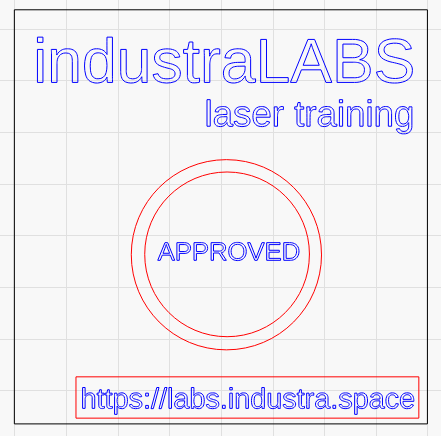
\includegraphics[scale=0.5]{imgs/lb_example.png}

\end{frame}


\begin{frame}
\frametitle{Operations}
\centering
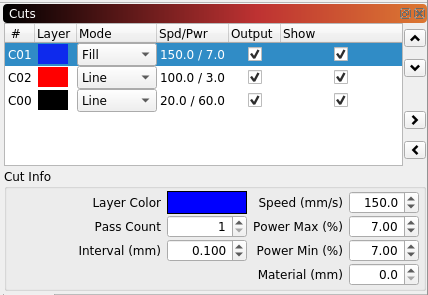
\includegraphics[scale=0.7]{imgs/lb_colors.png}

\end{frame}

\begin{frame}
\frametitle{Simulator}
\centering
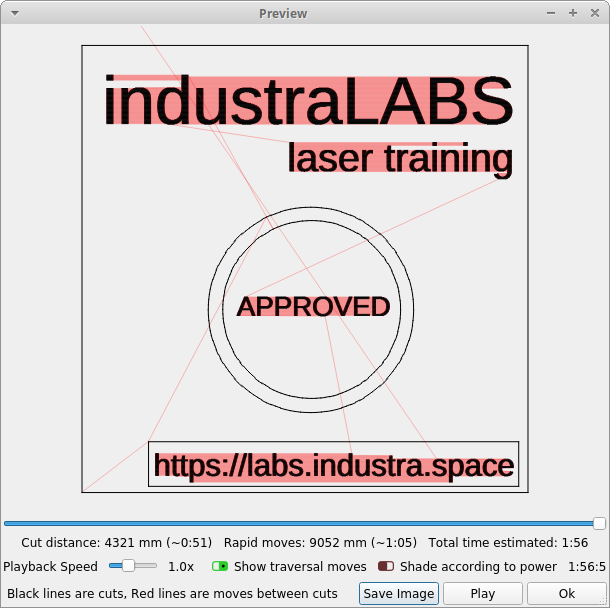
\includegraphics[scale=0.35]{imgs/lb_simulator.png}

\end{frame}






\section{Live Demo (Hardware)}
\begin{frame}
\frametitle{Live Demo}
\centering
\scalebox{13}{$\leftarrow$}


\end{frame}


\end{document}